\begin{figure}[t]\centering
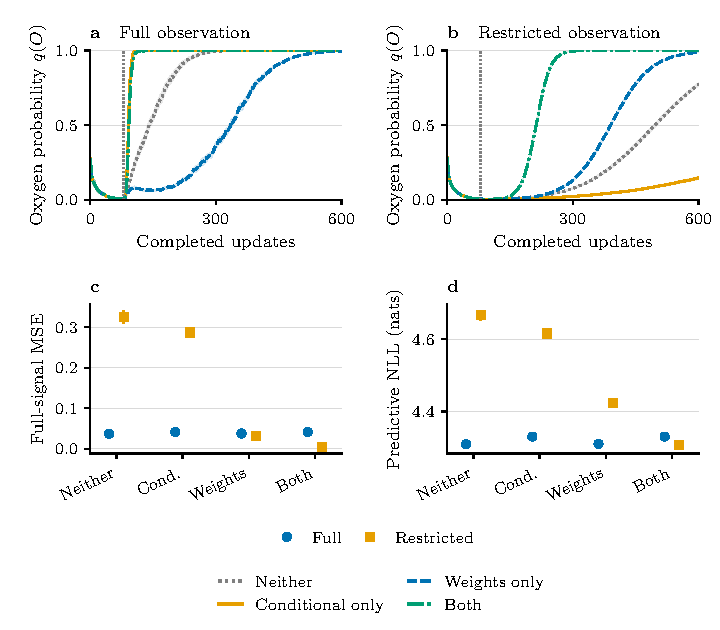
\includegraphics[width=\textwidth]{figures/fig_network_channels.pdf}
\caption{\textbf{Separate effects of the two communication channels.} Four arms share an 80-update fully observed history, then the mass signal changes from $-1$ to $+1$ (dotted line). Four agents retain full attention; twenty have weights $(1,.01,.01)$. The latter receive weak gas and mass evidence, not zero evidence. (a,b) Group-average oxygen probability. (c,d) Mean full-signal MSE and held-out mixture NLL over completed states 451--600, averaged within each observation group before averaging seeds; lower is better. Conditional exchange is uniform over 24 agents when enabled; model-weight exchange uses $\alpha_m=.02$ when enabled. $\omega=.9$, $\sigma_o=1$. The existing network seed set 0--49 is reused for paired extension, not independent confirmation of its three archived arms. Unless otherwise specified, ensemble curves and summary points summarize 50 paired seeds. Shading and error bars are pointwise 95\% percentile intervals from 2,000 whole-seed bootstrap resamples (analysis seed 20260920); they are neither ranges of agents nor simultaneous confidence bands. }\label{fig:fig_network_channels}\end{figure}

\begin{figure}[t]\centering
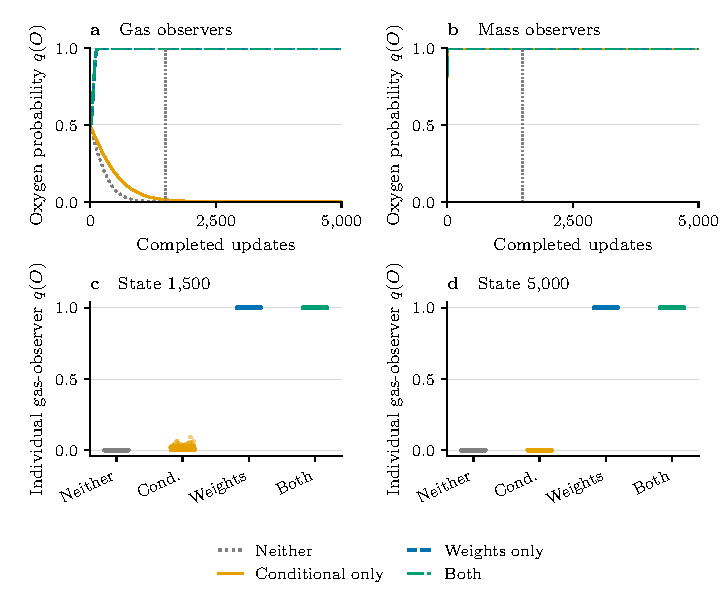
\includegraphics[width=\textwidth]{figures/fig_camp_channels.pdf}
\caption{\textbf{Communication channels and opposed account preferences.} Eight gas observers and eight mass observers receive private noisy measurements of the same constant observable signal $(1,1,1)$. (a,b) Group-average oxygen probability under four channel combinations. The dotted line marks the first reporting horizon, state 1,500. (c,d) Descriptive strip distributions of individual gas-observer probabilities at states 1,500 and 5,000, including all eight agents in each of 50 seeds (400 values per arm, dependent within seed). These distributions have no inferential bands. Fixed horizontal jitter separates coincident points and does not change probabilities. $\beta=.05$ is the total cross-group conditional weight; $\alpha_m=.02$ when model sharing is enabled; $\omega=.3$, $\sigma_o=.5$. Reference means and observation groups are identical across arms; scores accumulate without decay. Unless otherwise specified, ensemble curves and summary points summarize 50 paired seeds. Shading and error bars are pointwise 95\% percentile intervals from 2,000 whole-seed bootstrap resamples (analysis seed 20260920); they are neither ranges of agents nor simultaneous confidence bands. }\label{fig:fig_camp_channels}\end{figure}

\begin{figure}[t]\centering
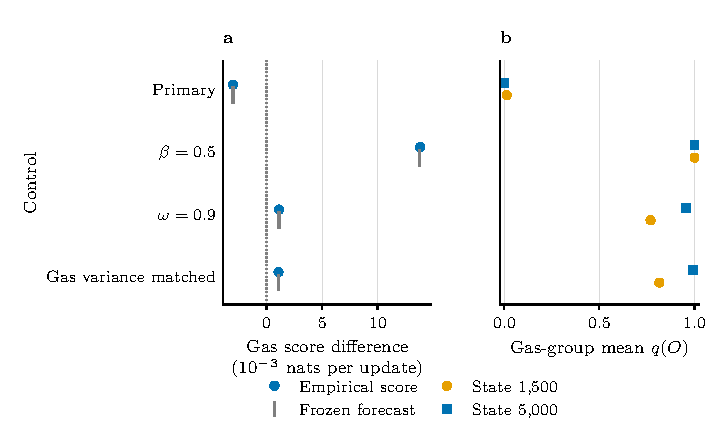
\includegraphics[width=\textwidth]{figures/fig_reference_diagnostics.pdf}
\caption{\textbf{Diagnostics of the small gas-score preference.} All four arms share conditional beliefs and retain private model weights. Primary settings are $\beta=.05$, $\omega=.3$, $\sigma_o=.5$. Each additional arm changes only the named setting; gas-variance matching changes the release gas residual from .5 to .5448, matching the reference gas marginal variance (.8648), not the full covariance or topology. (a) Oxygen-minus-release predictive score for gas observers, averaged over completed states 3,751--5,000. Grey ticks are stationary expectations supplied before this confirmation; they are not fitted to the runs and do not predict finite-time adoption exactly. (b) Gas-group mean oxygen probability at the two endpoints, distinct from window averages. Unless otherwise specified, ensemble curves and summary points summarize 50 paired seeds. Shading and error bars are pointwise 95\% percentile intervals from 2,000 whole-seed bootstrap resamples (analysis seed 20260920); they are neither ranges of agents nor simultaneous confidence bands. }\label{fig:fig_reference_diagnostics}\end{figure}

\begin{figure}[t]\centering
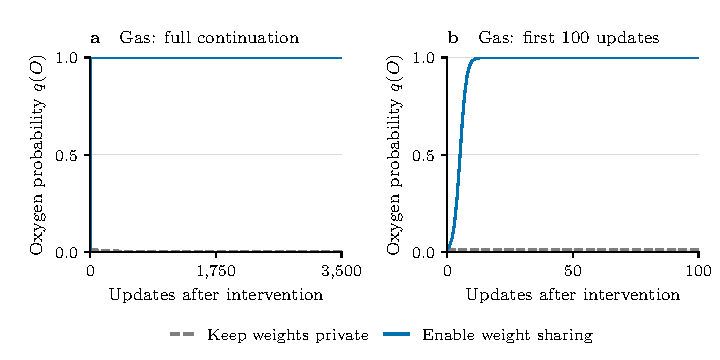
\includegraphics[width=\textwidth]{figures/fig_weight_sharing_intervention.pdf}
\caption{\textbf{A fixed-time intervention on model-weight communication.} Every primary conditional-only seed branches from its exact state 1,500: keep model weights private or enable $\alpha_m=.02$. Conditional sharing, attention, references and all future training and evaluation draws remain paired; no seed is selected by its outcome. Gas-group mean oxygen probability over (a) all 3,500 continuation updates and (b) the first 100 updates, a zoom specified before these runs using the expected rapid transfer of accumulated support. Mass-group probabilities remain at one to stored numerical precision; their full continuation and predictive outcomes appear in the intervention supplement. $\beta=.05$, $\omega=.3$, $\sigma_o=.5$. The origin is the common pre-intervention state. Conditional trajectories and direct score streams are unchanged by the intervention; probability-dependent predictions can change. Unless otherwise specified, ensemble curves and summary points summarize 50 paired seeds. Shading and error bars are pointwise 95\% percentile intervals from 2,000 whole-seed bootstrap resamples (analysis seed 20260920); they are neither ranges of agents nor simultaneous confidence bands. }\label{fig:fig_weight_sharing_intervention}\end{figure}

\begin{figure}[t]\centering
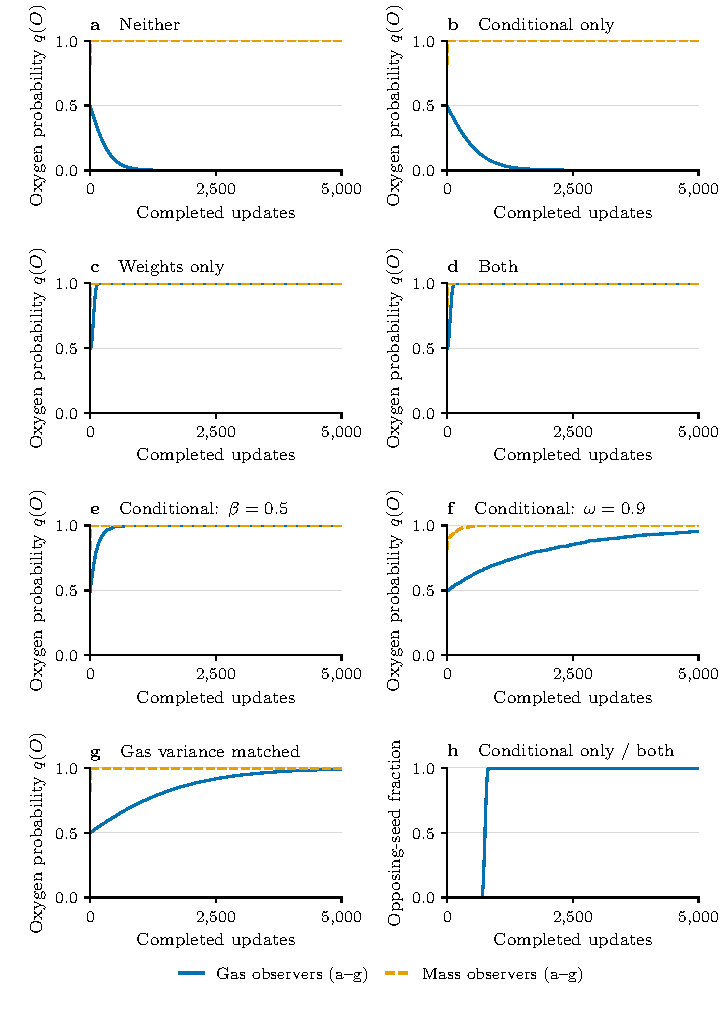
\includegraphics[width=\textwidth]{figures/fig_all_camp_conditions.pdf}
\caption{\textbf{All seven camp conditions over their full horizon.} (a--g) Gas- and mass-group mean oxygen probabilities. The three diagnostic arms change one primary conditional-only setting at a time. (h) Fraction of seeds whose gas-group mean probability is below .1 and mass-group mean is above .9, comparing conditional-only (blue solid) with both-channel communication (orange dashed). This is a statewise fraction, not the separate seed-pass criterion requiring 90\% occupancy in a reporting window. Unless otherwise specified, ensemble curves and summary points summarize 50 paired seeds. Shading and error bars are pointwise 95\% percentile intervals from 2,000 whole-seed bootstrap resamples (analysis seed 20260920); they are neither ranges of agents nor simultaneous confidence bands. }\label{fig:fig_all_camp_conditions}\end{figure}

\begin{figure}[t]\centering
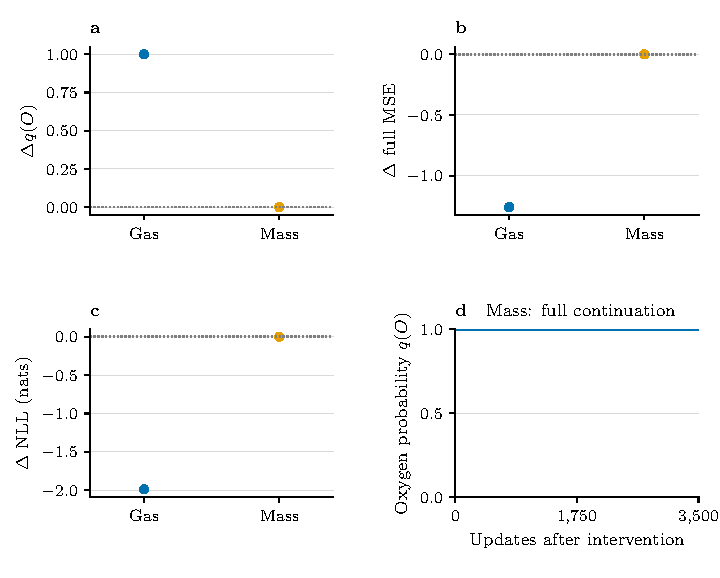
\includegraphics[width=\textwidth]{figures/fig_intervention_prediction.pdf}
\caption{\textbf{Paired predictive consequences of enabling model-weight sharing.} Each point is an enable-minus-keep difference, formed within each of the 50 seeds before aggregation. (a) Group-mean oxygen probability. (b) Full-signal mixture-mean MSE. (c) Held-out mixture NLL (nats per full observation). All three are averaged over completed states 3,751--5,000, separately for gas and mass observers. Negative predictive differences indicate improvement; a probability change alone does not establish improved prediction. (d) Full mass-group probability continuation: private (grey dashed) and shared (blue solid) weights overlap at one to stored numerical precision. Unless otherwise specified, ensemble curves and summary points summarize 50 paired seeds. Shading and error bars are pointwise 95\% percentile intervals from 2,000 whole-seed bootstrap resamples (analysis seed 20260920); they are neither ranges of agents nor simultaneous confidence bands. }\label{fig:fig_intervention_prediction}\end{figure}

\begin{figure}[t]\centering
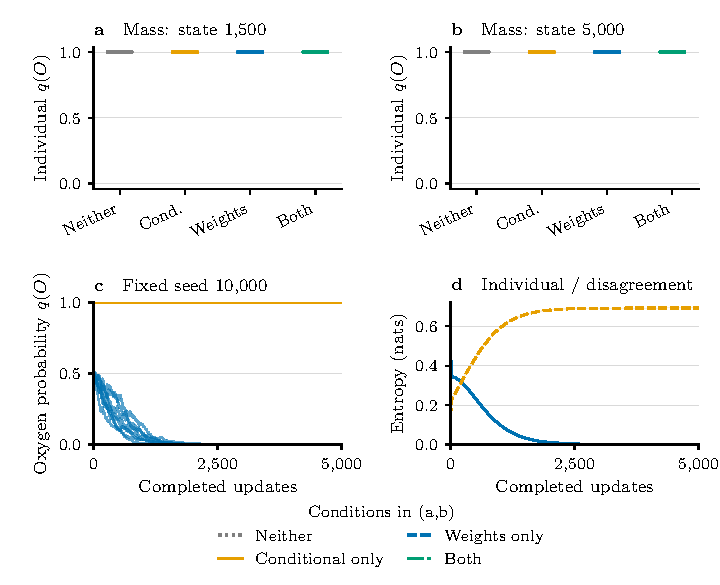
\includegraphics[width=\textwidth]{figures/fig_individual_and_uncertainty.pdf}
\caption{\textbf{Individual probabilities and uncertainty diagnostics.} (a,b) Individual mass-observer probability distributions for all four arms; strips show all 400 dependent agent values per arm, not 400 independent replications. Fixed horizontal jitter is for display only. (c) All 16 individual trajectories in the primary conditional-only condition for the prespecified illustrative seed 10,000; blue denotes gas and orange dashed mass. This seed is an illustration, not an inferential sample selected for a clear effect. (d) Within-seed average individual entropy (blue solid) and between-agent disagreement $H(\langle q_i\rangle)-\langle H(q_i)\rangle$ (orange dashed), then averaged across seeds. They distinguish uncertainty within agents from diversity between them. Entropy is displayed every ten updates without smoothing; summaries use every raw update. Unless otherwise specified, ensemble curves and summary points summarize 50 paired seeds. Shading and error bars are pointwise 95\% percentile intervals from 2,000 whole-seed bootstrap resamples (analysis seed 20260920); they are neither ranges of agents nor simultaneous confidence bands. }\label{fig:fig_individual_and_uncertainty}\end{figure}
